\section{Light sheet microscopy} 

Light sheet microscopy is an imaging technique used in biological physics and other fields to visualize materials -- often cells -- with high clarity and minimal phototoxicity.

Unlike conventional microscopes that illuminate the entire sample, light sheet microscopy utilizes a thin sheet of light to illuminate only a single plane at a time. 
The light sheet is generated using either cylindrical optics, precisely aligned in the focal plane of the detection objective. 

The excitation light is introduced perpendicular to the observation direction. By using a cylindrical 
lens, the expanded, collimated laser beam is focused in a single direction, forming a light disk 
at the focus that selectively illuminates a thin layer within the sample. In this light sheet
fluorescent dye molecules are exited, which can be observed. This process of illuminating only one plane significantly reduces photobleaching, making it good method for live-cell imaging and long-term observations. 

\begin{figure}[ht]
    \centering
    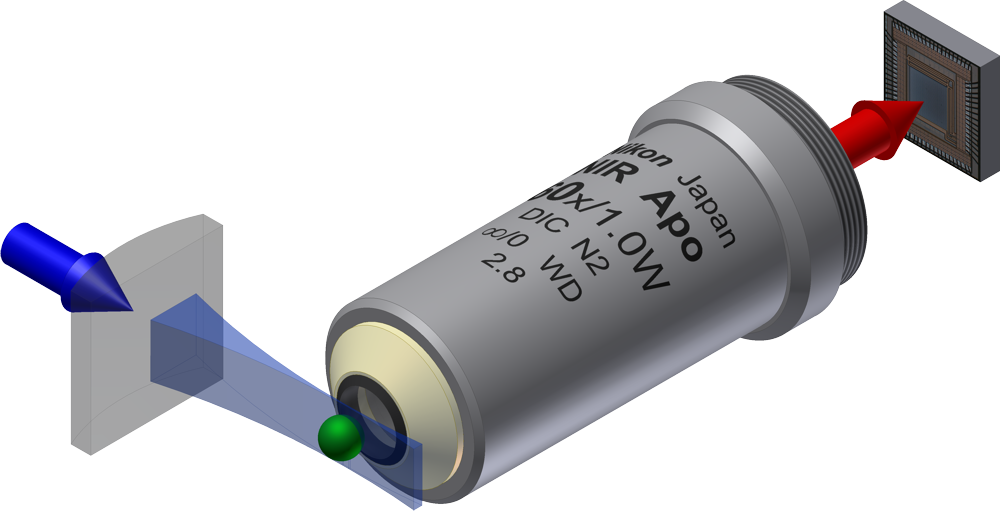
\includegraphics[width = 12cm]{Bilder/Theory/LSM.png}
    \caption[]{Schematic representation of a light sheet microscope\footnotemark}
    \label{fig:LSM}
\end{figure}\footnotetext{Jan Krieger (\url{https://commons.wikimedia.org/wiki/File:Spim_prinziple_en.svg}), „Spim prinziple en“, \url{https://creativecommons.org/licenses/by-sa/3.0/legalcode}}

A series of images (z-stack) can be recorded by linearly moving the sample through the light sheet. This allows a three-dimensional reconstruction of the sample. 

% In general, any micirocpy technique which introdices a contrast image by interaction between light and matter can be used for light sheet

Some advantages are the aforementioned reduced photobleaching, the high speed of scanning compared to confocal microscopy and the low setup costs. Futhermore, it is possible to 
access information below the diffraction limit as explained in \cref{sec:DDM}.
In contrast to this, the sample and setup adjustment can be time consuming and the data processing and 
can be get quite complex.  

